\documentclass[11pt]{article}
\usepackage[usenames]{color} %used for font color
\usepackage{amssymb} %maths
\usepackage{amsmath} %maths

\usepackage[no-math]{fontspec}
\usepackage{unicode-math}
\usepackage{libertinus}

\usepackage{pgf,xcolor}
\definecolor{itwm_blue_04}{HTML}{005A94}
\definecolor{itwm_red}{HTML}{C00000}

\usepackage{tikz}
\usetikzlibrary{shapes.misc, shadows, decorations}
\usetikzlibrary{backgrounds}
\usetikzlibrary{calc}
\usepackage{pgfplots}
\pgfplotsset{compat=newest}
\usepgfplotslibrary{fillbetween}
\usepackage{tikzpagenodes}
\begin{document}
\begin{align*}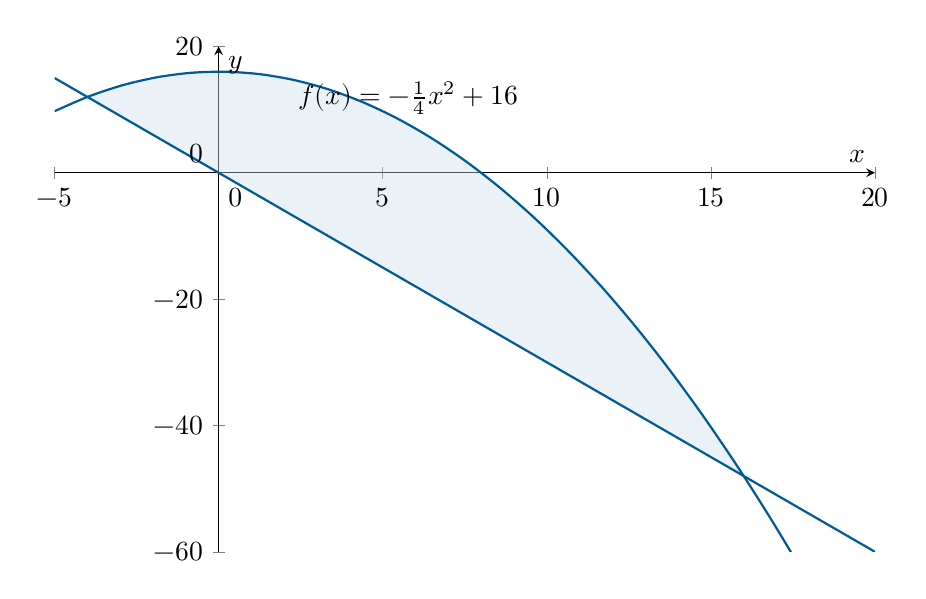
\begin{tikzpicture}
\begin{axis}[
    domain=-5:20,
    axis lines = center,
    xlabel = {$x$},
    ylabel = {$y$},
    height=8cm, width=12cm, 
    xmin=-5, xmax=20, ymin=-60, ymax=20, 
    xtick={-5,0,...,20},
    ytick={-60,-40,...,20},
    after end axis/.code={
        \path (axis cs:0,0) 
            node [anchor=north west,yshift=-0.075cm] {0}
            node [anchor=south east,xshift=-0.075cm] {0};
    }
]
\path [name path=xaxis]
      (\pgfkeysvalueof{/pgfplots/xmin},0) --
      (\pgfkeysvalueof{/pgfplots/xmax},0);
\addplot[draw=itwm_blue_04, smooth, thick, name path=f]{-1/4*x^2+16} node [pos=0.17,above] {$f(x)=-\frac{1}{4}x^2+16$};
\addplot[draw=itwm_blue_04, smooth, thick, name path=g]{-3*x};
\addplot[itwm_blue_04!20, opacity=0.4] fill between [of=f and g, soft clip={domain=-4:16}];
\end{axis}
\end{tikzpicture}
\end{align*}
\end{document}